\documentclass[]{beamer}
\mode<presentation>
{
  \usetheme{Warsaw}
  \definecolor{mcgarnet}{rgb}{0.38, 0, 0.08}
  \definecolor{mcgray}{rgb}{0.6, 0.6, 0.6}
  \setbeamercolor{structure}{fg=mcgarnet,bg=mcgray}
  %\setbeamercovered{transparent}
}


\usepackage[english]{babel}
\usepackage[latin1]{inputenc}
\usepackage{times}
\usepackage[T1]{fontenc}
\usepackage{tikz}
\usepackage{graphicx}
\usepackage{fancyvrb}
\usepackage{adjustbox}

\newcommand{\imagesource}[1]{{\centering\hfill\break\hbox{\scriptsize Image Source:\thinspace{\small\itshape #1}}\par}}

\title{Object Oriented Programming -- Implementation}


\author{Dr. Robert Lowe\\}

\institute[Maryville College] % (optional, but mostly needed)
{
  Division of Mathematics and Computer Science\\
  Maryville College
}

\date[]{}
\subject{}

\pgfdeclareimage[height=0.5cm]{university-logo}{images/Maryville-College}
\logo{\pgfuseimage{university-logo}}



\AtBeginSection[]
{
  \begin{frame}<beamer>{Outline}
    \tableofcontents[currentsection]
  \end{frame}
}


\begin{document}

\begin{frame}
  \titlepage
\end{frame}


% Structuring a talk is a difficult task and the following structure
% may not be suitable. Here are some rules that apply for this
% solution: 

% - Exactly two or three sections (other than the summary).
% - At *most* three subsections per section.
% - Talk about 30s to 2min per frame. So there should be between about
%   15 and 30 frames, all told.

% - A conference audience is likely to know very little of what you
%   are going to talk about. So *simplify*!
% - In a 20min talk, getting the main ideas across is hard
%   enough. Leave out details, even if it means being less precise than
%   you think necessary.
% - If you omit details that are vital to the proof/implementation,
%   just say so once. Everybody will be happy with that.

\begin{frame}{Address Book Design}
\begin{adjustbox}{max width=\textwidth, max totalheight=0.95\textheight}
    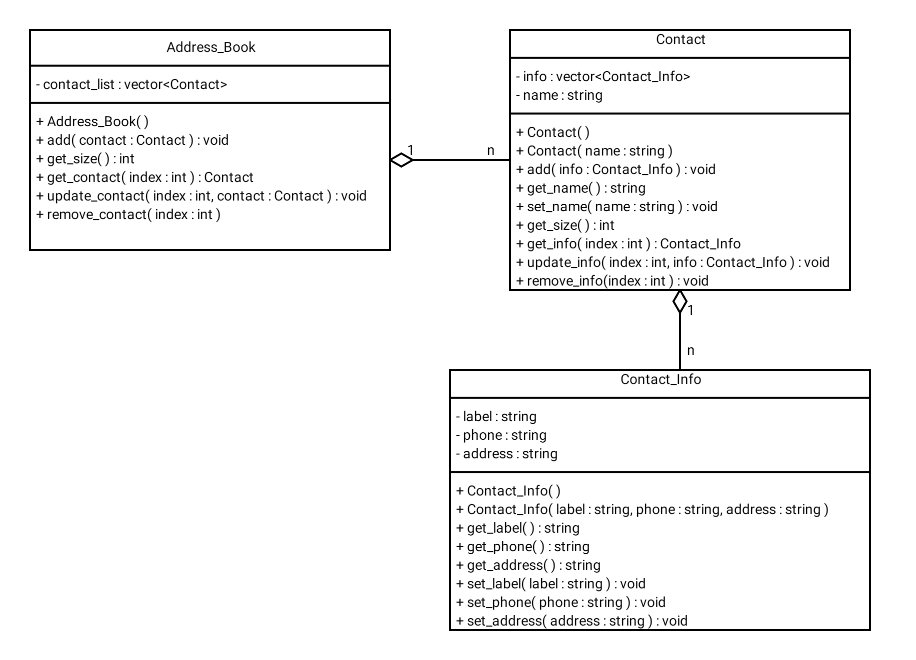
\includegraphics{images/AddressBook-Class.png}
\end{adjustbox}
\end{frame}

\begin{frame}[fragile]{Objects as Function Parameters}
    \begin{itemize}[<+(1)->]
        \item We typically pass objects by reference:
            \newline\verb!void load(Address_Book &book);!
        \item If an object is not going to be modified by a function,
            and the function only makes use of \texttt{const}
            functions, we typically use const references:
            \newline\verb!void set_name(const std::string& name);!
        \item The reasons we do this are threefold:
        \begin{itemize}
            \item Passing references is more efficient than copying objects.
            \item An object will usually need to maintain state across
                the function call. (If not, we use \texttt{const}).
            \item Polymorphism only works on on references and
                pointers (more on this later)!
        \end{itemize}
    \end{itemize}
\end{frame}

\begin{frame}[fragile]{Shadowing of Member Variables}
    \begin{BVerbatim}
//set the name of the contact
void Contact::set_name(const std::string& name)
{
    this->name = name;
}
    \end{BVerbatim}

    \begin{itemize}[<+(1)->]
    \item Sometimes we want to name a parameter the same thing as
        a member variable.
    \item We should do this!  Inventing other names would make the
        code less readable.
    \item The keyword \texttt{this} provides a pointer to the current
        object.
    \item We will talk about pointers next semester.  For now, we will
        just use \texttt{this} to distinguish the member from the
        parameter as shown above.
    \end{itemize}
\end{frame}

\begin{frame}[fragile]{Constructors with Parameters}
    \begin{itemize}[<+(1)->]
        \item We often want to initialize classes when we create them.
        \item We do this by specifying constructors with parameters.
        \item Most of the time, we have a no-argument constructor and
            one that requires arguments:
            \begin{itemize}
                \item \verb!Contact();!
                \item \verb!Contact(std::string name);!
            \end{itemize}
        \item We use this when we create an object:
            \newline\verb!Contact mom{"Mom"};!
    \end{itemize}
\end{frame}

\begin{frame}[fragile]{Lab Activity: Implement the Address Book}
    \begin{enumerate}
        \item \verb!mkdir labs/address!
        \item \verb!cp examples/21-OOP/* labs/address!
        \item Compile the program: \verb!g++ main.cpp contact.cpp iofun.cpp -o address!
        \item Run the program. Notice how it does very little.
        \item Implement the missing classes.
        \item Implement the missing functions in main.
    \end{enumerate}
\end{frame}

\end{document}


